\documentclass{standalone}
\usepackage{tikz}
\usetikzlibrary{matrix,chains,positioning,decorations.pathreplacing,arrows}
\usetikzlibrary{positioning,calc}
\begin{document}

\tikzset{%
  every neuron/.style={
    circle,
    draw,
    minimum size=1cm
  },
  neuron missing/.style={
    draw=none, 
    scale=4,
    text height=0.333cm,
    execute at begin node=\color{black}$\vdots$
  },
}

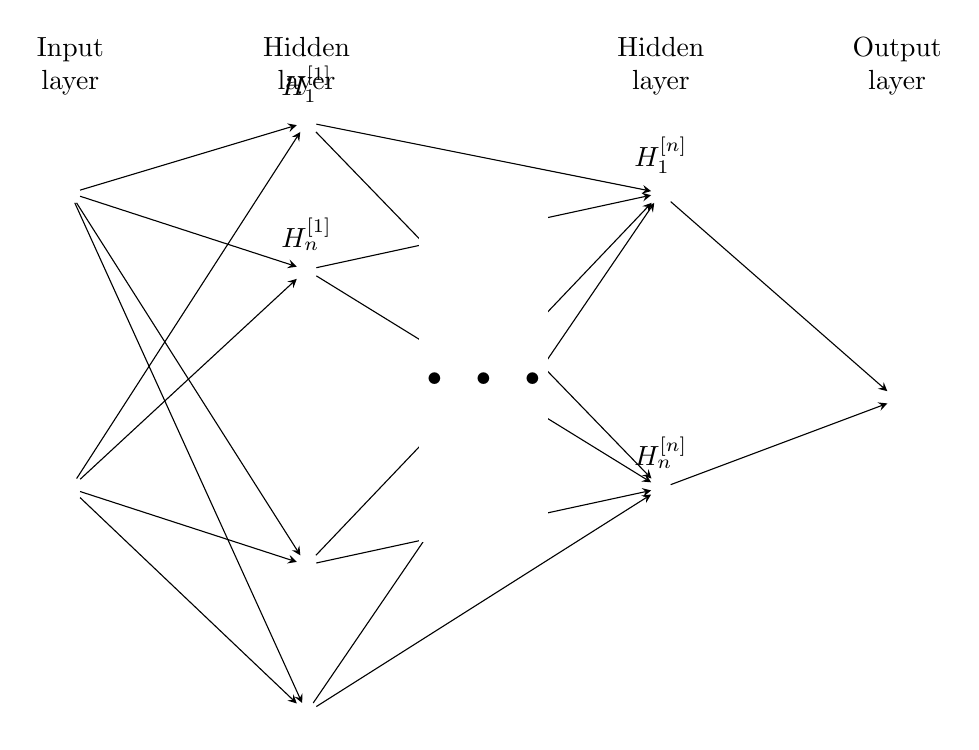
\begin{tikzpicture}[x=1.5cm, y=1.5cm, >=stealth]

\foreach \m/\l [count=\y] in {1,missing,2}
  \node [every neuron/.try, neuron \m/.try] (input-\m) at (0,2.5-\y*1.25) {};

\foreach \m [count=\y] in {1,2,missing,3,4}
  \node [every neuron/.try, neuron \m/.try ] (hidden1-\m) at (2,3.1-\y*1.25) {};

%\foreach \m [count=\y] in {1,missing,2}
%\node [every neuron/.try, neuron \m/.try ] (hidden1-\m) at (2,2-\y*1.25) {};

\foreach \m [count=\y] in {1,missing,2}
  \node [every neuron/.try, neuron \m/.try ] (hidden2-\m) at (5,2.5-\y*1.25) {};

\foreach \m [count=\y] in {1}
  \node [every neuron/.try, neuron \m/.try ] (output-\m) at (7,.5-\y) {};

% arrows to input labels
%\foreach \l [count=\i] in {1,2,3,n}
%  \draw [<-] (input-\i) -- ++(-1,0)
%    node [above, midway] {$I_\l$};

\foreach \l [count=\i] in {1,n}
  \node [above] at (hidden1-\i.north) {$H^{[1]}_\l$};

\foreach \l [count=\i] in {1,n}
  \node [above] at (hidden2-\i.north) {$H^{[n]}_\l$};

% arrows on output label
%\foreach \l [count=\i] in {1}
%  \draw [->] (output-\i) -- ++(1,0)
%    node [above, midway] {$O_\l$};


\foreach \i in {1,...,2}
  \foreach \j in {1,...,4}
    \draw [->] (input-\i) -- (hidden1-\j);

\foreach \i in {1,...,4}
  \foreach \j in {1,...,2}
    \draw [->] (hidden1-\i) -- (hidden2-\j);

    \foreach \i in {1,...,2}
    \foreach \j in {1}
    \draw [->] (hidden2-\i) -- (output-\j);

\node [align=center, above] at (0,2) {Input\\layer};
\node [align=center, above] at (2,2) {Hidden \\layer};
\node [align=center, above] at (5,2) {Hidden \\layer};
\node [align=center, above] at (7,2) {Output \\layer};

% lonsome dots
\node[fill=white,scale=4,inner xsep=0pt,inner ysep=5mm] at ($(hidden1-2)!.5!(hidden2-2)$) {$\dots$};

\end{tikzpicture}
\end{document}